% Deck Demo Day (Jumat 23 Okt 2026): 7 menit pitch + live demo, 5 menit QnA.
% Fokus: sistem yang kami jual; maks 3 angka kunci di slide utama (angka lengkap di lampiran dan naskah.md).
% Template panitia (logo, pita teal) dari ../template-pitch-deck-demo-day.pptx; kembarannya demoday.pptx (buat_pptx.py).
% Bangun: ml/.venv/bin/python demo-day/buat_aset.py (angka + gambar TikZ), lalu latexmk -xelatex demoday.tex
% Video tertanam diputar di Okular, Adobe Reader, atau pdfpc; viewer lain menampilkan poster.
\documentclass[aspectratio=169, 10pt]{beamer}

\usepackage[indonesian]{babel}
\usepackage{fontspec}
% Tahoma (font template) tidak ada di Linux; DejaVu Sans Condensed punya bentuk humanis dan lebar yang mirip.
\IfFontExistsTF{Tahoma}{\setsansfont{Tahoma}}{\setsansfont{DejaVu Sans Condensed}}
\newfontfamily\judulfont{DejaVu Sans}[BoldFont={DejaVu Sans Bold}, Ligatures=TeX]
\setmonofont{DejaVu Sans Mono}[Scale=0.8]
\usepackage{tikz}
\usetikzlibrary{positioning,arrows.meta,calc}
\usepackage{booktabs,tabularx,array,colortbl}
\usepackage{pifont}

\definecolor{gelap}{HTML}{15242B}
\definecolor{teal}{HTML}{285052}
\definecolor{amber}{HTML}{E8A317}
\definecolor{muda}{HTML}{DCE8E8}
\definecolor{abu}{HTML}{8A9499}
\definecolor{teks}{HTML}{1E2B30}
\colorlet{izma}{teal}\colorlet{genis}{teal!70!green}\colorlet{alif}{amber!85!black}\colorlet{shania}{gelap!80}
\colorlet{lama}{abu}\colorlet{merah}{red!65!black}\colorlet{krem}{muda}\colorlet{espresso}{gelap}
% Gaya bersama diagram (dipakai laporan progress dan deck). Warna anggota sama dengan jobdesc.tex.
\providecolor{izma}{RGB}{31,94,170}
\providecolor{genis}{RGB}{40,130,70}
\providecolor{alif}{RGB}{190,90,20}
\providecolor{shania}{RGB}{140,60,150}
\providecolor{lama}{RGB}{110,110,110}
\providecolor{merah}{RGB}{185,40,40}
\tikzset{
  kotak/.style={draw, rounded corners=3pt, align=center, font=\footnotesize, inner sep=4pt, line width=0.8pt, minimum height=0.9cm},
  milik/.style={kotak, draw=#1, fill=#1!10},
  abu/.style={kotak, draw=lama, fill=black!4},
  panah/.style={-{Stealth[length=2mm]}, line width=0.7pt, draw=black!70},
  putus/.style={panah, dashed},
  label/.style={font=\scriptsize\itshape, text=black!70, fill=white, inner sep=1pt},
  wadah/.style={draw=#1!60, fill=#1!4, rounded corners=5pt, line width=0.6pt, inner sep=6pt},
}

\newcommand{\diagram}[1]{\input{../../diagram/#1.tex}}
\newcommand{\datafile}[1]{../../data/#1}
% Dibuat otomatis oleh buat_aset.py dari ml/results/energi_harian.json; jangan diedit manual.
\newcommand{\energiTurbin}{270}
\newcommand{\energiQa}{187}
\newcommand{\energiQb}{377}
\newcommand{\hariEnergi}{140}
\newcommand{\raspiWh}{71}
\newcommand{\chipWh}{4,1}
\newcommand{\raspiPersen}{26}
\newcommand{\chipPersen}{1,5}
\newcommand{\raspiPersenA}{19}
\newcommand{\raspiPersenB}{38}
\newcommand{\raspiPersenNum}{26.3}
\newcommand{\chipPersenNum}{1.5}
\newcommand{\hematKwh}{24}
\newcommand{\kaliHemat}{17}
\newcommand{\jRaspi}{182}
\newcommand{\jChip}{10,4}
\newcommand{\periodeEnergi}{2026-03-31--2026-10-20}

\graphicspath{{gambar/}{aset/}{../../../proposal/gambar/}{../}}
% \filmtertanam{lebar}{tinggi}{poster}{video}{aspek "w h"}: poster + anotasi /Movie (XeLaTeX/xdvipdfmx).
\newcommand{\filmtertanam}[5]{\makebox[#1][l]{\special{pdf:ann width #1 height #2 depth 0pt <</Subtype/Movie /Border [0 0 0]
    /T (video) /Movie <</F (#4) /Aspect [#5]>> /A <</ShowControls true /Mode /Repeat>> >>}%
  \includegraphics[width=#1,height=#2]{#3}}}
% Video yang belum tentu ada (rekaman dashboard, papan chip dari tim): placeholder sampai file tersedia.
\newcommand{\filmatau}[6]{\IfFileExists{#4}{\filmtertanam{#1}{#2}{#3}{#4}{#5}}%
  {\tikz\node[draw=abu, dashed, rounded corners=3pt, minimum width=#1, minimum height=#2, align=center, text width=#1, font=\fontsize{7}{8.5}\selectfont, text=abu]{#6};}}

% ---------- tema: latar template panitia ----------
\setbeamertemplate{navigation symbols}{}
\setbeamertemplate{background canvas}{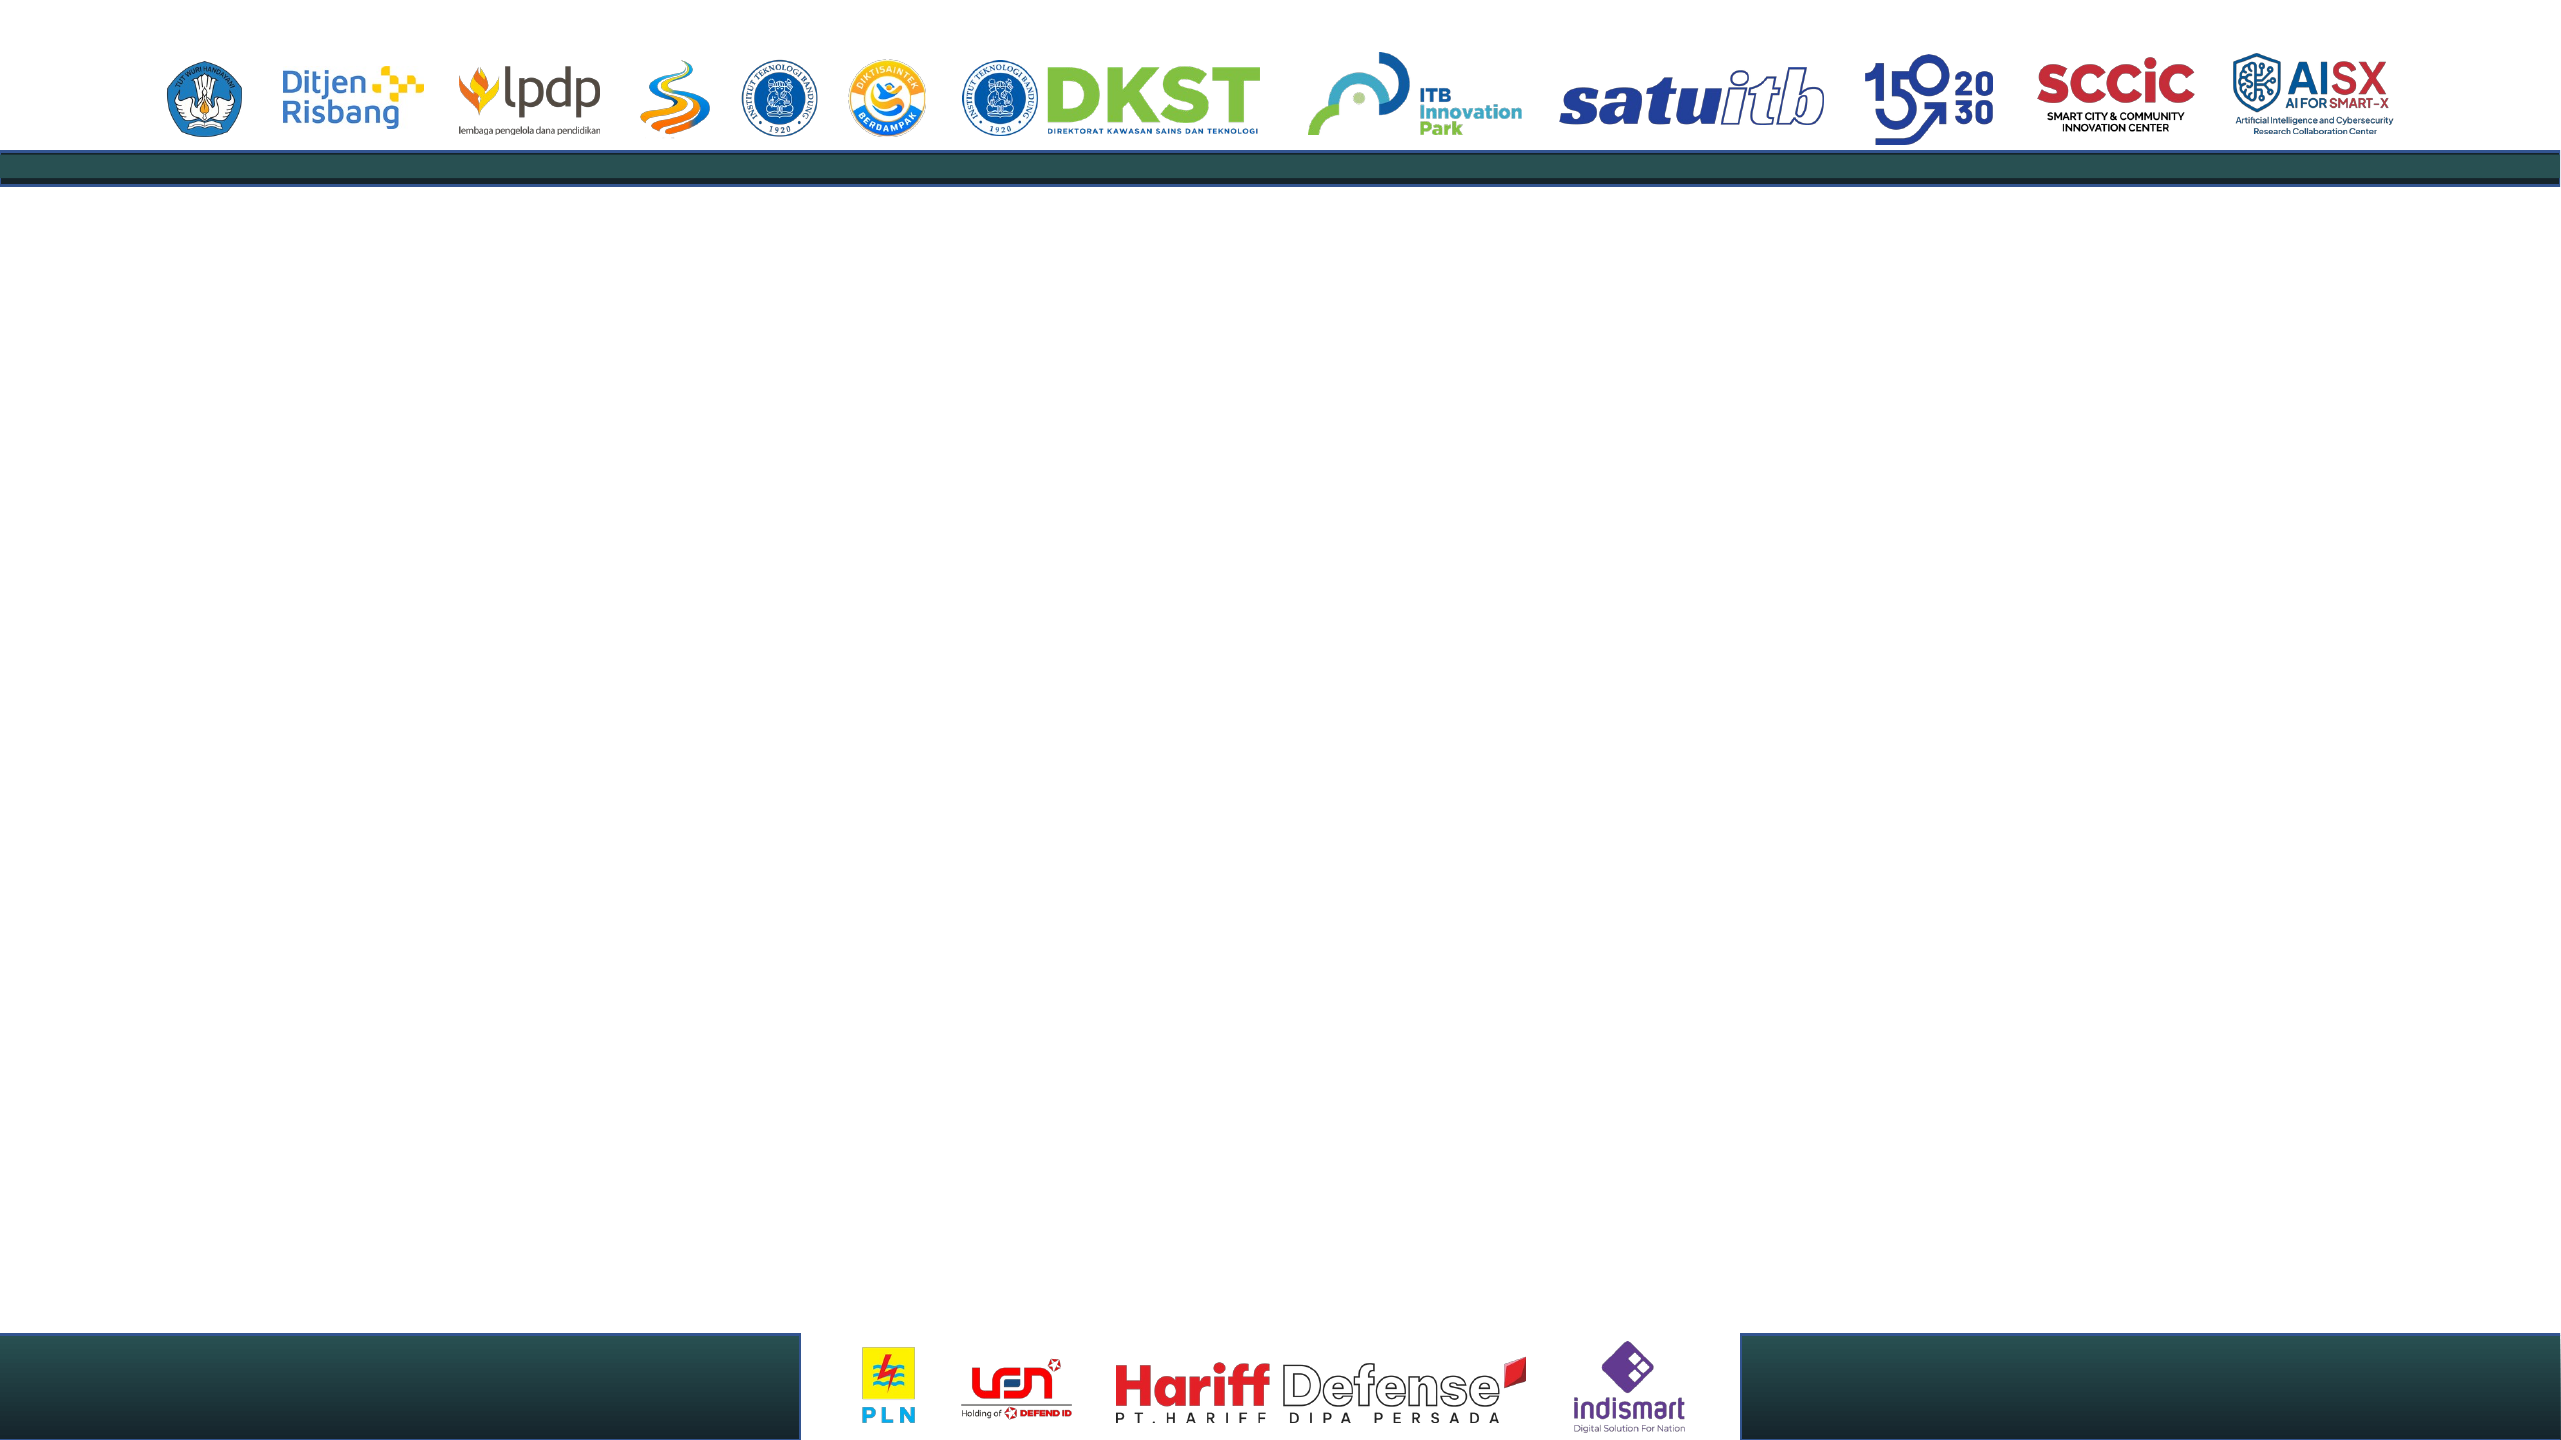
\includegraphics[width=\paperwidth,height=\paperheight]{latar-template.png}}
\setbeamercolor{normal text}{fg=teks}
\setbeamercolor{structure}{fg=teal}
\setbeamertemplate{itemize item}{\color{amber}\scriptsize$\blacktriangleright$}
\setbeamertemplate{enumerate item}{\color{teal}\bfseries\insertenumlabel.}
\setlength{\leftmargini}{1.1em}
\setbeamertemplate{headline}{\vspace*{1.22cm}}
\newcommand{\vidbaris}[6]{\noindent\begin{minipage}[c]{3.75cm}\filmatau{3.75cm}{2.11cm}{#1}{#2}{#3}{#4}\end{minipage}\hspace{6pt}%
\begin{minipage}[c]{2.45cm}\raggedright\fontsize{7}{8.5}\selectfont\textbf{#5}\\{\color{abu}#6}\end{minipage}\par}
\newcommand{\logopelat}[1]{\tikz\node[fill=white, rounded corners=2pt, inner sep=2pt]{
\includegraphics[height=#1]{logo-cita.png}};}
\setbeamertemplate{footline}{%
  \begin{tikzpicture}[remember picture, overlay]
    \node[anchor=west, inner sep=0] (lg) at ([xshift=0.3cm, yshift=0.33cm]current page.south west) {\logopelat{0.28cm}};
    \node[anchor=west, text=white, font=\tiny] at ([xshift=4pt]lg.east) {Tim Chitato \textbullet{} Wind Edge Chip};
    \node[anchor=east, text=white, font=\tiny\bfseries] at ([xshift=-0.35cm, yshift=0.33cm]current page.south east) {\insertframenumber};
  \end{tikzpicture}\vspace*{0.68cm}}
\setbeamertemplate{frametitle}{%
  {\color{amber}\fontsize{7}{8}\selectfont\bfseries\insertframesubtitle}\par\vspace{2pt}
  {\color{gelap}\judulfont\fontsize{14}{16}\selectfont\bfseries\insertframetitle}\par\vspace{2pt}}
\newcommand{\kriteria}[1]{\hfill{\mdseries\color{abu}Rubrik: #1}}
\newcommand{\pitaatas}{([yshift=-1.19cm]current page.north west)}
\newcommand{\pitabawah}{([yshift=0.67cm]current page.south east)}
\newcommand{\pitagelap}{\fill[left color=gelap, right color=teal] \pitaatas rectangle \pitabawah;}

\begin{document}
\hyphenpenalty=10000 \exhyphenpenalty=10000 \sloppy

% ====================================================================== 1 JUDUL (0:00)
\begin{frame}[plain]
\begin{tikzpicture}[remember picture, overlay]
  \pitagelap
  \begin{scope}
    \clip ([xshift=-6.6cm, yshift=-1.19cm]current page.north east) rectangle \pitabawah;
    \node[anchor=north east, inner sep=0] at ([yshift=0.4cm]current page.north east) {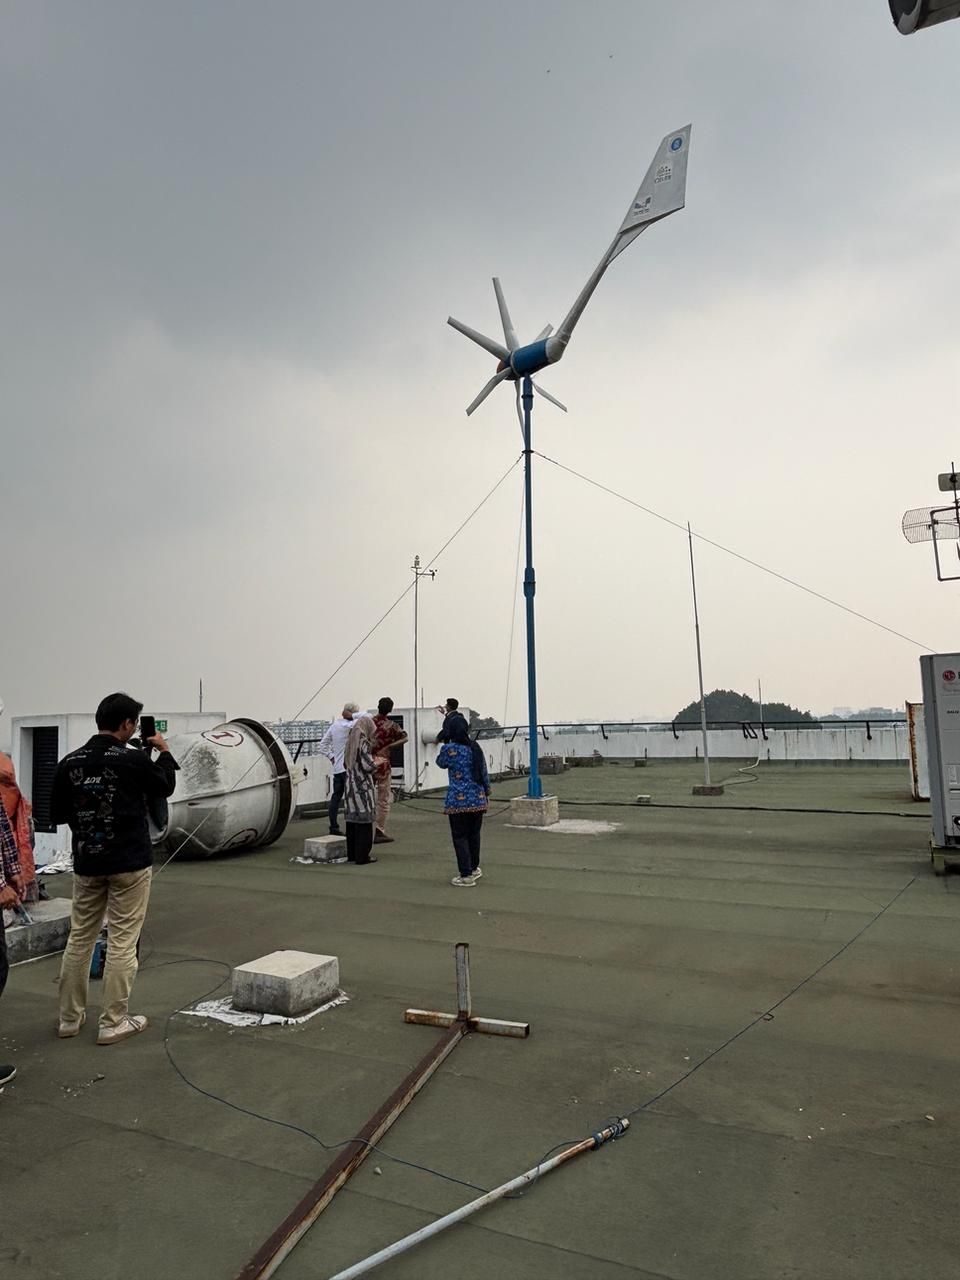
\includegraphics[width=6.6cm]{foto-turbin-atap.jpeg}};
  \end{scope}
  \fill[amber] ([xshift=-6.65cm, yshift=-1.19cm]current page.north east) rectangle ([xshift=-6.6cm, yshift=0.67cm]current page.south east);
  \node[anchor=north west, inner sep=0] at ([xshift=0.8cm, yshift=-1.5cm]current page.north west) {\logopelat{0.42cm}};
  \node[anchor=north west, text width=8.3cm, text=white] at ([xshift=0.8cm, yshift=-2.15cm]current page.north west) {%
    {\color{amber}\fontsize{6.5}{8}\selectfont\bfseries DEEPTECH FOR SMART-X HACKATHON 2026 \textbullet{} RENEWABLE ENERGY}\\[6pt]
    {\fontsize{12}{14}\selectfont\bfseries Tim Chitato:}\\[1pt]
    {\judulfont\fontsize{25}{29}\selectfont\bfseries Wind Edge Chip}\\[6pt]
    {\fontsize{10.5}{13.5}\selectfont Sistem pintar \textcolor{amber}{\textbf{hemat daya}} untuk turbin angin: chip rancangan sendiri yang memprediksi, mengatur baterai\textsuperscript{*}, dan menjaga turbin.}\\[9pt]
    {\fontsize{7.3}{9.8}\selectfont\color{muda}
     \textbf{Anggota:} Izma Alhazmi Herdian (ketua) \textbullet{} Genis Gusvian Hartanto\\Alif Muhammad Rizky \textbullet{} Shania Argiliana\\
     \textbf{Pembimbing:} Ir.\ Estiyanti Ekawati, M.T., Ph.D.\\[4pt]\textsuperscript{*}\,kontrol baterai: pengembangan selanjutnya}};
  \node[anchor=south west, text=muda, font=\fontsize{7}{8}\selectfont] at ([xshift=0.8cm, yshift=0.82cm]current page.south west) {Institut Teknologi Bandung \textbar{} 21--23 Oktober 2026};
  \node[anchor=south east, fill=amber, text=gelap, font=\fontsize{7}{8}\selectfont\bfseries, inner sep=3pt] at ([xshift=-0.2cm, yshift=0.85cm]current page.south east)
    {LIVE \textbullet{} turbin atap Gedung CRIMSE ITB};
\end{tikzpicture}
\end{frame}

% ====================================================================== 2 KONDISI SAAT INI (0:15)
\begin{frame}{Turbin butuh ``otak'' pengatur energi}{01 \textbullet{} KONDISI SAAT INI\kriteria{problem-solution fit 20\%}}
\begin{columns}[c]
\begin{column}{0.27\linewidth}\centering
\filmtertanam{2.5cm}{4.42cm}{poster-video.jpg}{../video-turbin.mp4}{480 848}\\[1pt]
{\fontsize{6.5}{7.5}\selectfont\color{abu}turbin TA kami di atap CRIMSE ITB (klik untuk memutar)}
\end{column}
\begin{column}{0.7\linewidth}
\begin{tikzpicture}[font=\footnotesize, every node/.style={align=left}]
  \node[fill=muda, rounded corners=5pt, text width=8.9cm, inner sep=6pt] (a) {\textbf{\color{teal}Energi angin tumbuh}\\RUPTL 2025--2034 menargetkan +7,2 GW pembangkit angin; PLTB kecil dipasang di rumah, kawasan, dan daerah terpencil};
  \node[fill=amber!30, rounded corners=5pt, text width=8.9cm, inner sep=6pt, below=0.22cm of a] (b) {\textbf{\color{gelap}Turbin perlu dipantau dan diatur}\\kapan mengisi baterai, kapan membuang kelebihan ke dump load, kapan memakai PLN};
  \node[fill=gelap, text=white, rounded corners=5pt, text width=8.9cm, inner sep=6pt, below=0.22cm of b] {\textbf{\color{amber}Di turbin TA kami (sejak Maret 2026)}\\``otaknya'' Raspberry Pi 4 + internet + Google Sheets; keluaran ke dump load 35\,$\Omega$, berikutnya baterai 12\,V 50\,Ah};
\end{tikzpicture}
\end{column}
\end{columns}
\end{frame}

% ====================================================================== 3 PROBLEM (0:40)
\begin{frame}{Masalahnya: ``otak'' turbin mahal, boros, rapuh}{02 \textbullet{} PROBLEM\kriteria{problem-solution fit 20\%}}
\centering
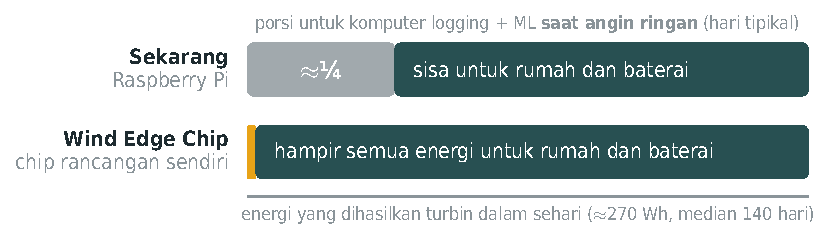
\includegraphics[width=0.78\linewidth]{anggaran.pdf}\\[6pt]
\begin{columns}[T]
\begin{column}{0.32\linewidth}\footnotesize\textbf{\color{gelap}Mahal}\\Satu set komputer mini $\pm$Rp3,3 jt per turbin.\end{column}
\begin{column}{0.32\linewidth}\footnotesize\textbf{\color{gelap}Boros}\\Memakan $\approx$\textonequarter{} energi turbin \textbf{saat angin ringan}, padahal tugasnya hanya mencatat dan memprediksi.\end{column}
\begin{column}{0.32\linewidth}\footnotesize\textbf{\color{gelap}Rapuh}\\Internet putus $\to$ Raspi reboot, data dan prediksi hilang (2.787 kali, Apr--Okt).\end{column}
\end{columns}
\end{frame}

% ====================================================================== 4 PROBLEM STATEMENT (1:05)
\begin{frame}[plain]
\begin{tikzpicture}[remember picture, overlay]
  \pitagelap
  \node[anchor=north west, text=amber, font=\fontsize{7.5}{9}\selectfont\bfseries] at ([xshift=1.6cm, yshift=-1.65cm]current page.north west) {03 \textbullet{} PROBLEM STATEMENT};
  \node[anchor=north west, text=amber, font=\judulfont\fontsize{40}{40}\selectfont\bfseries] at ([xshift=0.45cm, yshift=-2.1cm]current page.north west) {``};
  \node[anchor=north west, text width=13.2cm, text=white, font=\judulfont\fontsize{17}{23}\selectfont\bfseries] at ([xshift=1.6cm, yshift=-2.3cm]current page.north west)
    {Bagaimana membuat ``otak'' turbin yang \textcolor{amber}{murah}, \textcolor{amber}{hemat daya}, tetap jalan \textcolor{amber}{tanpa internet}, dan bisa \textcolor{amber}{mengatur baterai}?};
  \draw[amber, line width=1pt] ([xshift=1.6cm, yshift=1.95cm]current page.south west) -- ++(2cm,0);
  \node[anchor=south west, text width=13.4cm, text=muda, font=\fontsize{8}{10}\selectfont] at ([xshift=1.6cm, yshift=0.95cm]current page.south west)
    {\textbf{Siapa:} pemilik PLTB rumah menengah ke atas dan perusahaan dengan banyak turbin \quad\textbullet\quad \textbf{Kendala:} komputer mahal dan boros, internet putus, angin tak pasti};
\end{tikzpicture}
\end{frame}

% ====================================================================== 5 KENAPA ESP32 + FPGA (1:20)
\begin{frame}{Kenapa ESP32 + chip FPGA, bukan komputer mini?}{04 \textbullet{} PILIHAN TEKNOLOGI\kriteria{inovasi 15\% \textbullet{} TKDN 10\%}}
\centering
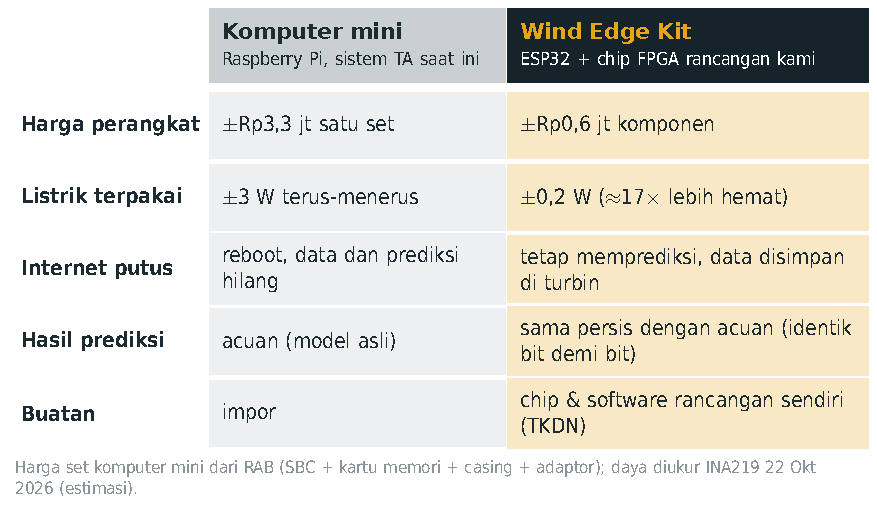
\includegraphics[height=5.3cm]{banding.pdf}
\end{frame}

% ====================================================================== 5 SISTEM KAMI (1:30)
\begin{frame}{Sistem kami: Wind Edge Kit + Platform}{05 \textbullet{} SOLUTION\kriteria{inovasi 15\% \textbullet{} fungsional 25\%}}
\centering
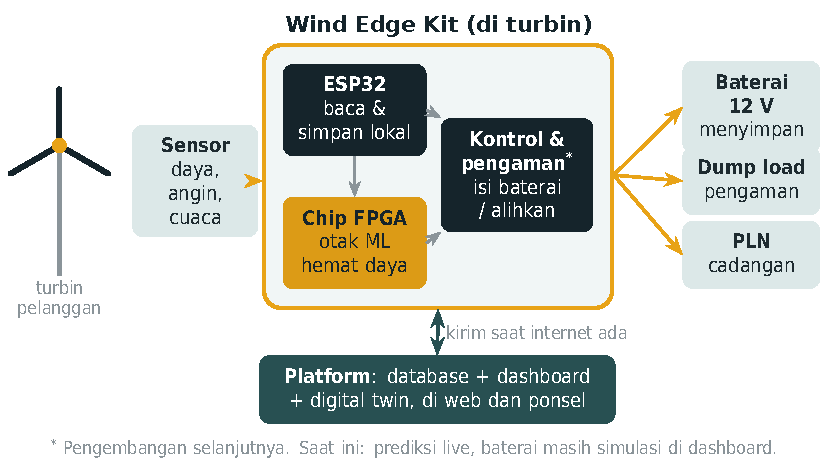
\includegraphics[height=5.35cm]{sistem.pdf}
\end{frame}

% ====================================================================== 6 YANG KAMI JUAL (2:05)
\begin{frame}{Yang kami jual: sistem, bukan turbin}{06 \textbullet{} PRODUK\kriteria{hilirisasi 10\%}}
\centering
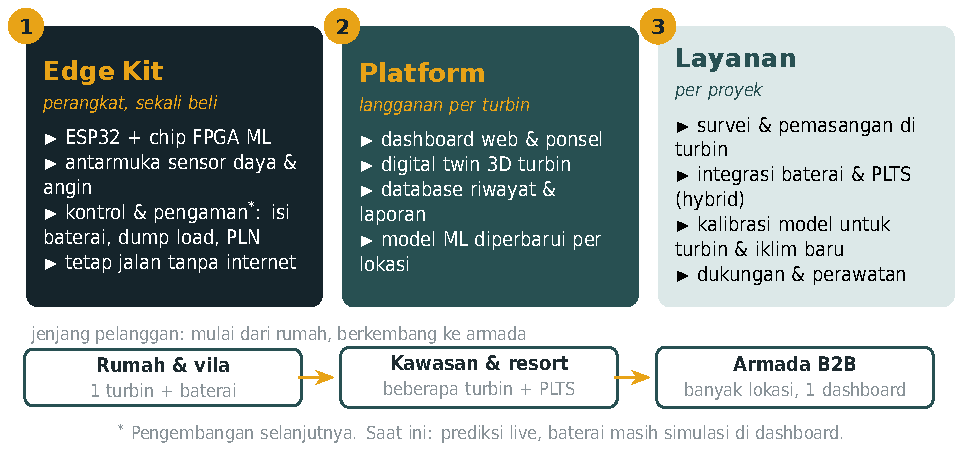
\includegraphics[height=5.45cm]{paket.pdf}
\end{frame}

% ====================================================================== 7 CARA KERJA (2:40)
\begin{frame}{Satu hari bersama Wind Edge Chip}{07 \textbullet{} CARA SISTEM BEKERJA UNTUK PELANGGAN\kriteria{dampak 15\%}}
\centering
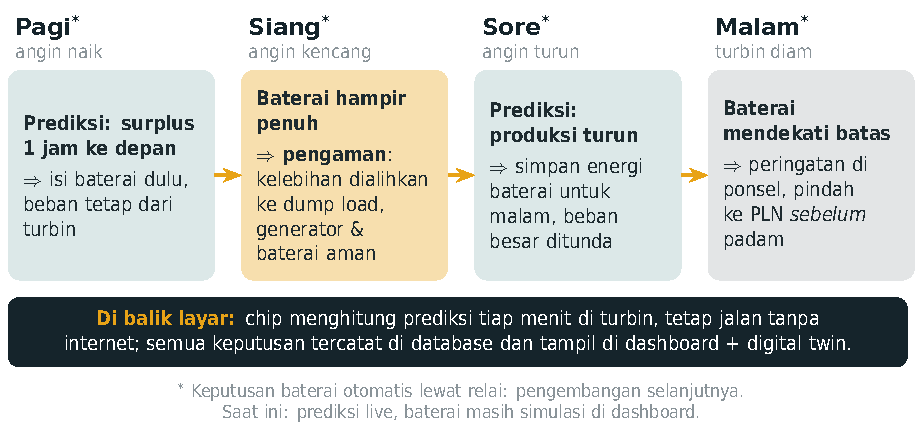
\includegraphics[height=5.35cm]{alur.pdf}
\end{frame}

% ====================================================================== 8 DEMO LIVE (3:10)
\begin{frame}{Demo live: sistem jalan sekarang}{08 \textbullet{} LIVE DEMO \textbullet{} 2 MENIT\kriteria{fungsional prototipe 25\%}}
\begin{columns}[T]
\begin{column}{0.5\linewidth}
\small
\begin{enumerate}\setlength{\itemsep}{2pt}
  \item \textbf{Dashboard}: turbin detik ini dan prediksi 1 jam.
  \item \textbf{Chip di plant}: terpasang di turbin, menjawab tiap menit, ``identik dengan CPU''.
  \item \textbf{Baterai\textsuperscript{*} \& status}: isi baterai 1 jam lagi, kondisi turbin.
  \item \textbf{Hemat daya}: Raspberry Pi vs chip, diukur live.
\end{enumerate}
\vspace{2pt}
\begin{tikzpicture}
  \node[inner sep=0] (q) {
\includegraphics[width=1.45cm]{qr-dashboard.png}};
  \node[right=5pt of q, text width=3.9cm, font=\fontsize{8}{10}\selectfont, align=left] {pindai untuk ikut membuka di ponsel\\[2pt]{\ttfamily\fontsize{6}{7}\selectfont citaitb.com:1880/\\dashboard/hackathon}};
\end{tikzpicture}
\end{column}
\begin{column}{0.47\linewidth}
\vidbaris{video-dashboard.jpg}{video-dashboard.mp4}{1280 720}{rekaman dashboard}{Rekaman dashboard}{cadangan bila internet putus (20 detik, klik untuk memutar)}
\vspace{5pt}
\vidbaris{video-chip.jpg}{video-chip.mp4}{1024 576}{papan chip}{Papan chip di plant}{ESP32-S3 + Tang Nano 4K FPGA + sensor daya INA219}
\vspace{4pt}
{\raggedright\fontsize{6.5}{8}\selectfont\color{abu}\textsuperscript{*} Pengembangan selanjutnya. Saat ini: prediksi live, baterai masih simulasi di dashboard.\par}
\end{column}
\end{columns}
\end{frame}

% ====================================================================== 9 BUKTI (5:10)
\begin{frame}{Bukan janji: sudah diukur}{09 \textbullet{} BUKTI\kriteria{fungsional 25\% \textbullet{} problem-solution fit 20\%}}
\centering
\vspace*{6pt}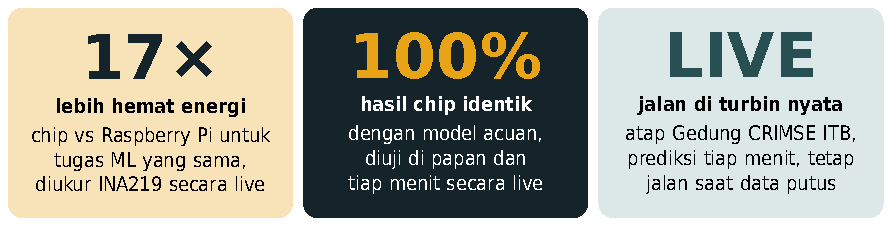
\includegraphics[width=\linewidth]{bukti.pdf}\\[10pt]
{\small Prediksi chip mengikuti daya aktual turbin (lampiran C) \textbullet{} angka lengkap dan sumbernya di lampiran A}
\end{frame}

% ====================================================================== 11 LEBIH MURAH, LEBIH BANYAK ENERGI (5:40)
\begin{frame}{Lebih murah, lebih banyak energi}{10 \textbullet{} BISNIS\kriteria{hilirisasi 10\% \textbullet{} dampak 15\%}}
\centering
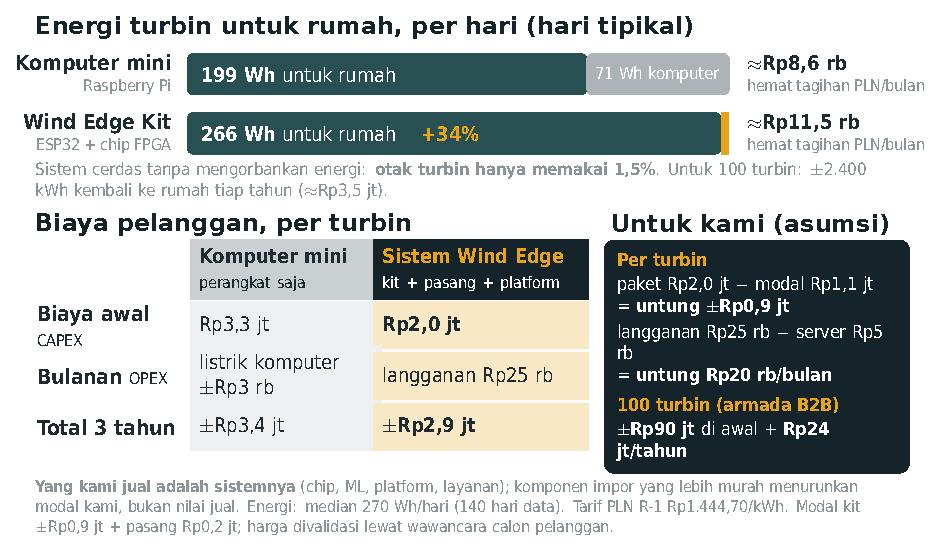
\includegraphics[height=5.5cm]{uang.pdf}
\end{frame}

% ====================================================================== 10 PASAR (5:40)
\begin{frame}{Mulai dari rumah, berkembang ke armada}{11 \textbullet{} PASAR\kriteria{hilirisasi 10\% \textbullet{} dampak 15\%}}
\centering
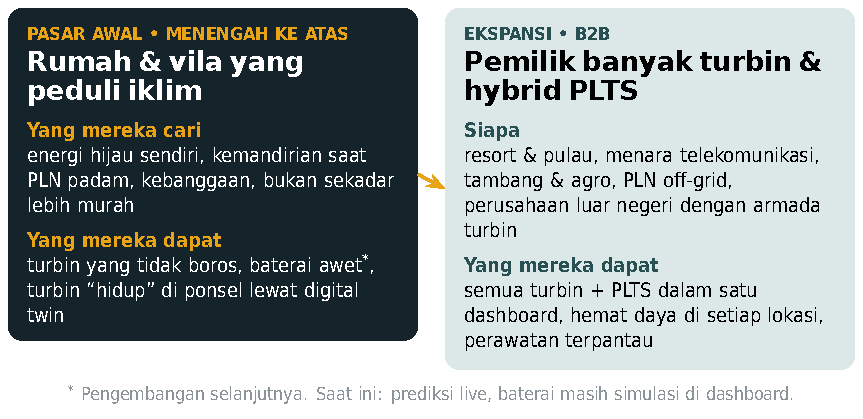
\includegraphics[height=4.25cm]{pasar.pdf}\\[5pt]
{\footnotesize\textbf{\color{teal}Pendapatan:} Edge Kit (sekali beli) \textbullet{} langganan Platform per turbin \textbullet{} layanan pemasangan \& integrasi PLTS}
\end{frame}

% ====================================================================== 11 KENAPA KAMI (6:15)
\begin{frame}{Kenapa kami, dan langkah berikutnya}{12 \textbullet{} INOVASI, TKDN \& PETA JALAN\kriteria{inovasi 15\% \textbullet{} TKDN 10\%}}
\begin{columns}[T]
\begin{column}{0.24\linewidth}\begin{tikzpicture}\node[fill=gelap, text=white, rounded corners=4pt, text width=3.0cm, minimum height=1.35cm, align=left, inner sep=5pt, font=\fontsize{8}{10}\selectfont]{\textbf{\color{amber}Chip \& IP sendiri}\\RTL, firmware, model: TKDN, jalur ke ASIC};\end{tikzpicture}\end{column}
\begin{column}{0.24\linewidth}\begin{tikzpicture}\node[fill=teal, text=white, rounded corners=4pt, text width=3.0cm, minimum height=1.35cm, align=left, inner sep=5pt, font=\fontsize{8}{10}\selectfont]{\textbf{\color{amber}Tanpa internet}\\prediksi \& kontrol\textsuperscript{*} tetap jalan di turbin};\end{tikzpicture}\end{column}
\begin{column}{0.24\linewidth}\begin{tikzpicture}\node[fill=muda, rounded corners=4pt, text width=3.0cm, minimum height=1.35cm, align=left, inner sep=5pt, font=\fontsize{8}{10}\selectfont]{\textbf{\color{teal}Satu kit lengkap}\\sensor sampai dashboard + digital twin};\end{tikzpicture}\end{column}
\begin{column}{0.24\linewidth}\begin{tikzpicture}\node[fill=amber!30, rounded corners=4pt, text width=3.0cm, minimum height=1.35cm, align=left, inner sep=5pt, font=\fontsize{8}{10}\selectfont]{\textbf{\color{gelap}Pengaman bawaan\textsuperscript{*}}\\baterai \& generator dijaga otomatis};\end{tikzpicture}\end{column}
\end{columns}
\vspace{4pt}
\centering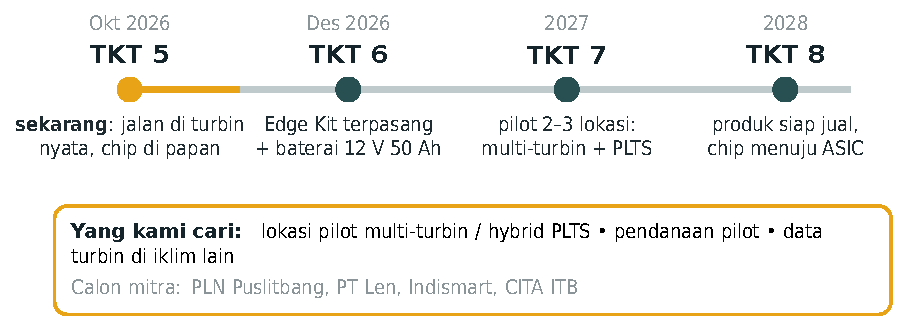
\includegraphics[height=2.75cm]{peta.pdf}\\[1pt]
{\fontsize{7}{8.5}\selectfont\color{abu}\textsuperscript{*} Pengembangan selanjutnya. Saat ini: prediksi live, baterai masih simulasi di dashboard.}
\end{frame}

% ====================================================================== 12 PENUTUP (6:40)
\begin{frame}[plain]
\begin{tikzpicture}[remember picture, overlay]
  \pitagelap
  \node[anchor=north west, text=amber, font=\fontsize{7.5}{9}\selectfont\bfseries] at ([xshift=1.0cm, yshift=-1.65cm]current page.north west) {RINGKASAN};
  \node[anchor=north west, text=white, font=\judulfont\fontsize{22}{26}\selectfont\bfseries, text width=9.6cm] at ([xshift=1.0cm, yshift=-2.0cm]current page.north west)
    {Otak hemat daya\\\textcolor{amber}{di setiap turbin.}};
  \node[anchor=north west, text=white, text width=9.6cm, font=\fontsize{9}{12.5}\selectfont] at ([xshift=1.0cm, yshift=-3.95cm]current page.north west) {%
    \textcolor{amber}{\ding{51}}\ \textbf{Sistem lengkap}: Edge Kit + Platform + Layanan.\\
    \textcolor{amber}{\ding{51}}\ \textbf{\kaliHemat\texttimes{} lebih hemat}, hasil chip identik, jalan di turbin nyata.\\
    \textcolor{amber}{\ding{51}}\ Mulai dari \textbf{rumah}, berkembang ke \textbf{armada B2B} dan \textbf{hybrid PLTS}.};
  \node[anchor=south west, text=muda, text width=10.4cm, font=\fontsize{7.5}{9.5}\selectfont] at ([xshift=1.0cm, yshift=0.95cm]current page.south west) {%
    {\color{white}\bfseries\small Tim Chitato: \emph{``Angin boleh berubah, keputusanmu tidak lagi menebak.''}}\\[3pt]
    Izma Alhazmi Herdian \textbullet{} Genis Gusvian Hartanto \textbullet{} Alif Muhammad Rizky \textbullet{} Shania Argiliana\\Pembimbing: Ir.\ Estiyanti Ekawati, M.T., Ph.D.};
  \node[anchor=east, fill=white, inner sep=4pt, rounded corners=3pt] (q) at ([xshift=-1.2cm, yshift=0.55cm]current page.east) {
\includegraphics[width=2.4cm]{qr-dashboard.png}};
  \node[below=3pt of q, text=white, font=\fontsize{6}{7.5}\selectfont, align=center] (u) {Dashboard live\\\ttfamily citaitb.com:1880/dashboard/hackathon};
  \node[below=6pt of u, inner sep=0] {\logopelat{0.5cm}};
\end{tikzpicture}
\end{frame}

% ====================================================================== LAMPIRAN (QnA)
\appendix
\begin{frame}{Angka lengkap dan sumbernya}{LAMPIRAN A}
\fontsize{6.8}{8.2}\selectfont
\renewcommand{\arraystretch}{1.12}
\begin{tabularx}{\linewidth}{@{}>{\raggedright}p{3.6cm} >{\raggedright}p{4.4cm} >{\raggedright\arraybackslash}X@{}}
\toprule
Besaran & Nilai & Sumber \\
\midrule
Energi turbin per hari & median \energiTurbin\ Wh (separuh hari \energiQa--\energiQb\ Wh) & register PZEM bersih, \hariEnergi\ hari (\texttt{energi\_harian.json}) \\
Konsumsi Raspberry Pi / papan chip & 2,96 W / 0,17 W & INA219 22 Okt, rata-rata seluruh papan, tanpa multimeter \\
Porsi energi turbin untuk komputer & Raspi \raspiPersen\% (\raspiPersenA--\raspiPersenB\%), chip \chipPersen\% & \raspiWh\ Wh vs \chipWh\ Wh per hari \\
Energi per prediksi & \jRaspi\ J vs \jChip\ J ($\approx$\kaliHemat\texttimes) & pencatat Raspi 22 Okt, 1 prediksi per menit \\
Hemat per turbin & $\approx$\hematKwh\ kWh per tahun & (2,96 $-$ 0,17) W $\times$ 24 jam $\times$ 365 \\
Inferensi chip identik & 5.373/5.373, 309 siklus & uji HIL 21 Okt (\texttt{docs/demo/hil-2026-10-21.txt}) \\
Akurasi prediksi 1 jam & MAE 5,48 W vs persistence 8,67 W ($-$37\%) & uji 1--20 Okt (\texttt{ml/results/mlp.json}) \\
Tahan gangguan & sensor daya mati: MAE 5,14 W (normal 5,07 W); 20\% data hilang: prediksi ada 97,7\% waktu & \texttt{test\_tanpa\_pzem.js}, \texttt{test\_celah.js} \\
Raspi reboot karena internet & 2.787 kali (Apr--Okt) & \texttt{log\_reboot.txt} Raspi \\
\bottomrule
\end{tabularx}
\end{frame}

\begin{frame}{Energi harian turbin dan cara menghitungnya}{LAMPIRAN B}
\begin{columns}[c]
\begin{column}{0.58\linewidth}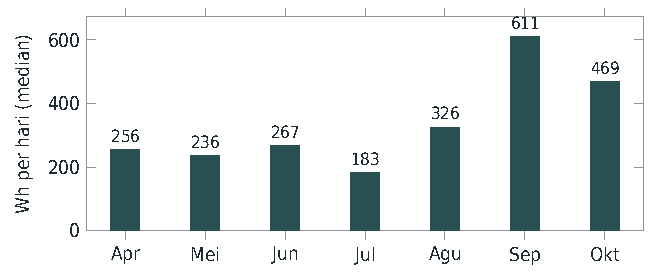
\includegraphics[width=\linewidth]{energi.pdf}\end{column}
\begin{column}{0.4\linewidth}\fontsize{8}{10}\selectfont
\begin{itemize}
  \item ``Total Energy'' di dashboard = register PZEM sejak reset terakhir, bukan per hari.
  \item Energi harian = kenaikan register yang dibersihkan (reset, flicker, lompatan tak wajar dibuang); baris OFF = 0 W.
  \item Pada data tanpa celah, register = integrasi daya (rasio 1,01). Saat Raspi reboot, PZEM tetap menghitung sehingga register lebih lengkap.
\end{itemize}
\end{column}
\end{columns}
\end{frame}

\begin{frame}{Contoh prediksi 1 jam: chip vs daya aktual}{LAMPIRAN C}
\centering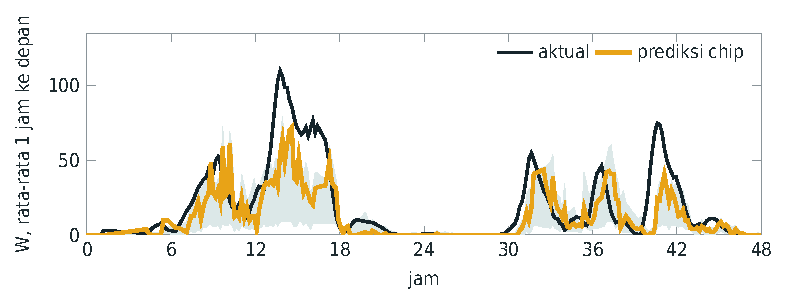
\includegraphics[width=0.88\linewidth]{prediksi.pdf}\\[2pt]
{\footnotesize Data uji Oktober (tidak dipakai melatih). Area muda = rentang 80\%.}
\end{frame}

\begin{frame}{Alur data dan database}{LAMPIRAN C2}
\centering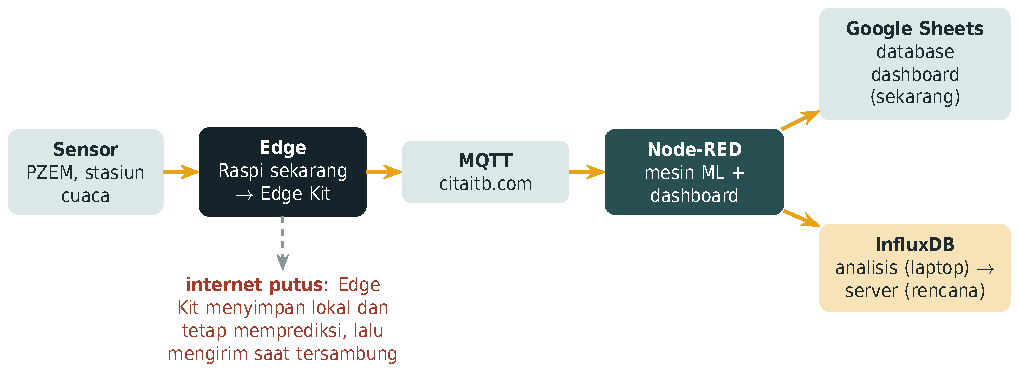
\includegraphics[width=\linewidth]{alurdata.pdf}
\end{frame}

\begin{frame}{Arsitektur teknis}{LAMPIRAN D}
\centering\resizebox{!}{5.3cm}{\diagram{arsitektur}}
\end{frame}

\begin{frame}{Chip: akselerator MAC4 rancangan sendiri}{LAMPIRAN E}
\centering\resizebox{!}{4.3cm}{\diagram{mac4}}\\[6pt]
\footnotesize Paket UART 19 B \texttt{[AA 55, 16 fitur, CRC-8]} $\to$ balasan 7 B, 921600 bps; 309 siklus per prediksi.
\end{frame}

\begin{frame}{Perbandingan metode prediksi (uji 1--20 Okt)}{LAMPIRAN F}
\centering
\IfFileExists{\datafile{tabel_benchmark_deck.tex}}{\scalebox{0.62}{\begin{minipage}[t]{1.6\linewidth}\input{\datafile{tabel_benchmark_deck.tex}}\end{minipage}}}{}
\end{frame}

\begin{frame}{Inferensi live: Raspberry Pi vs chip}{LAMPIRAN G}
\centering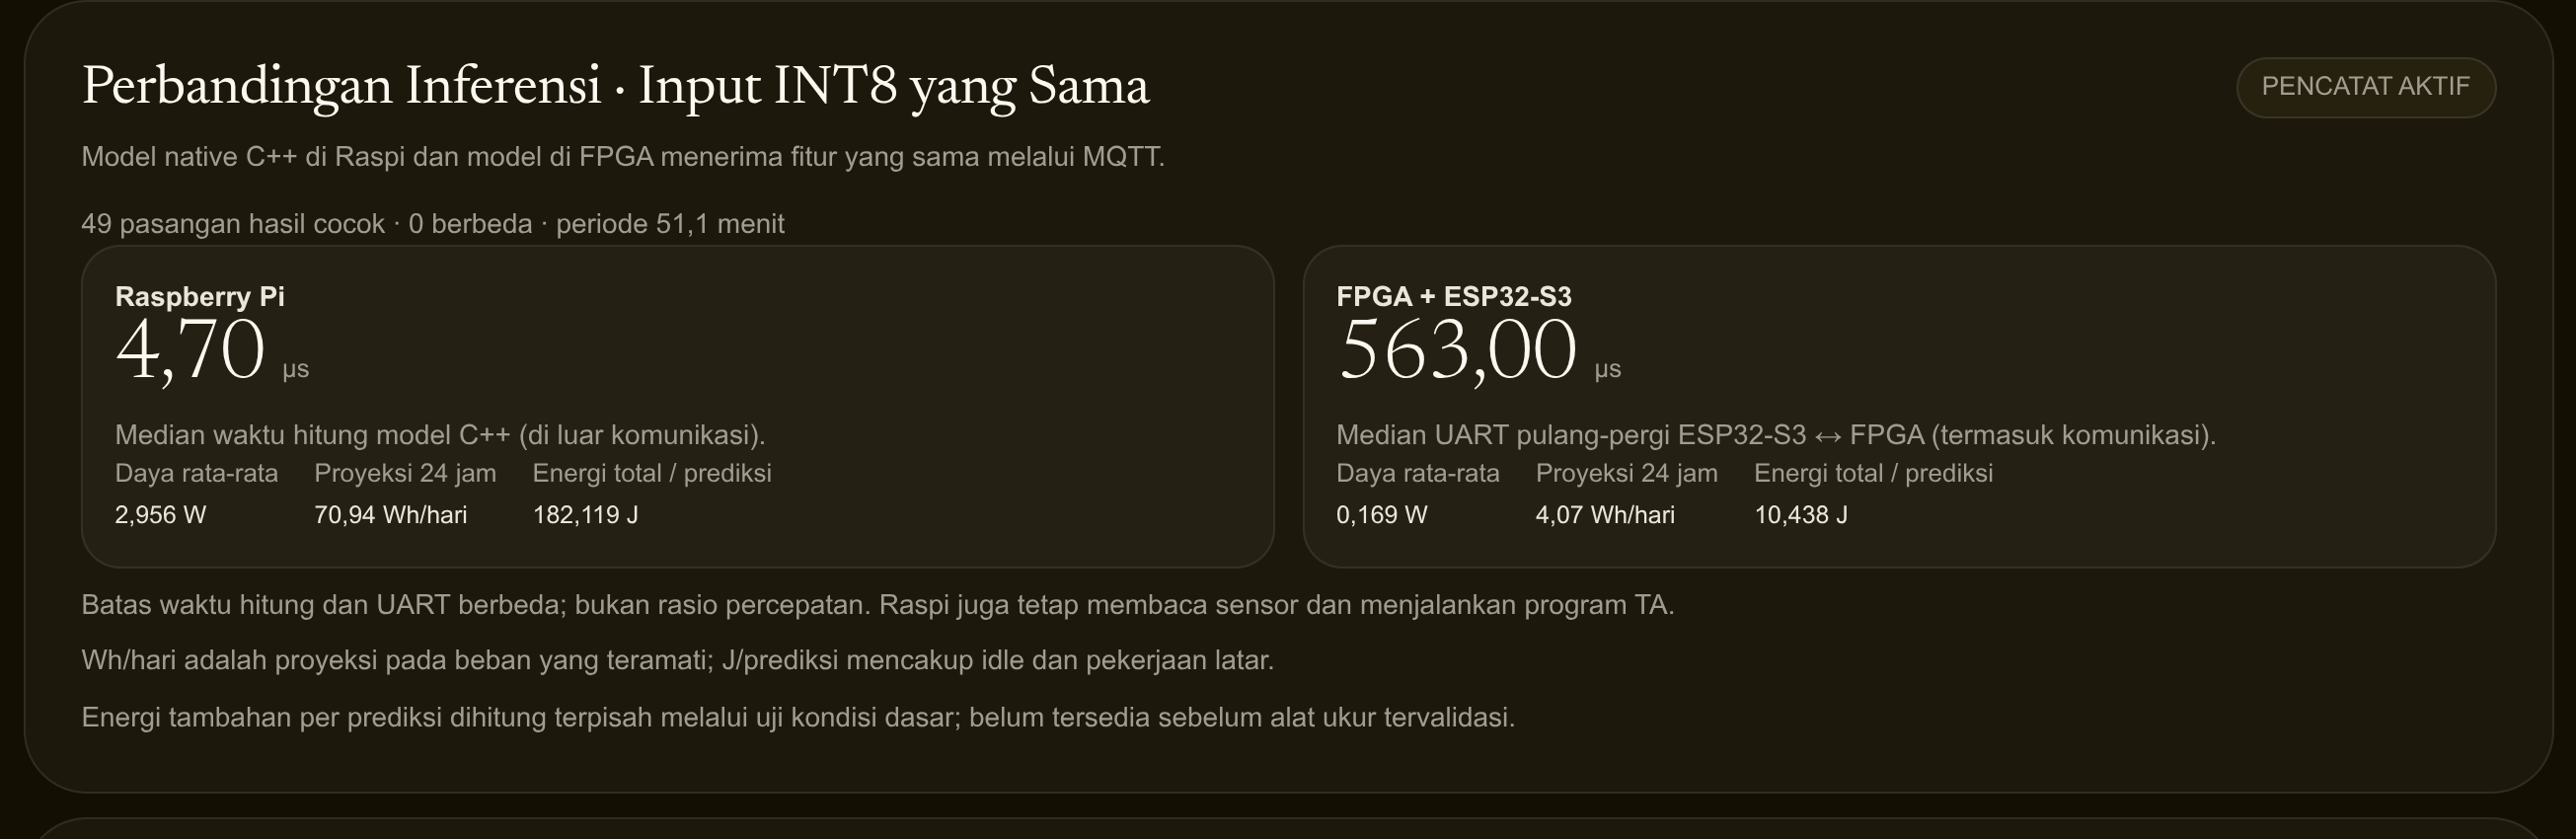
\includegraphics[height=2.3cm]{dash-banding.png}\\[3pt]
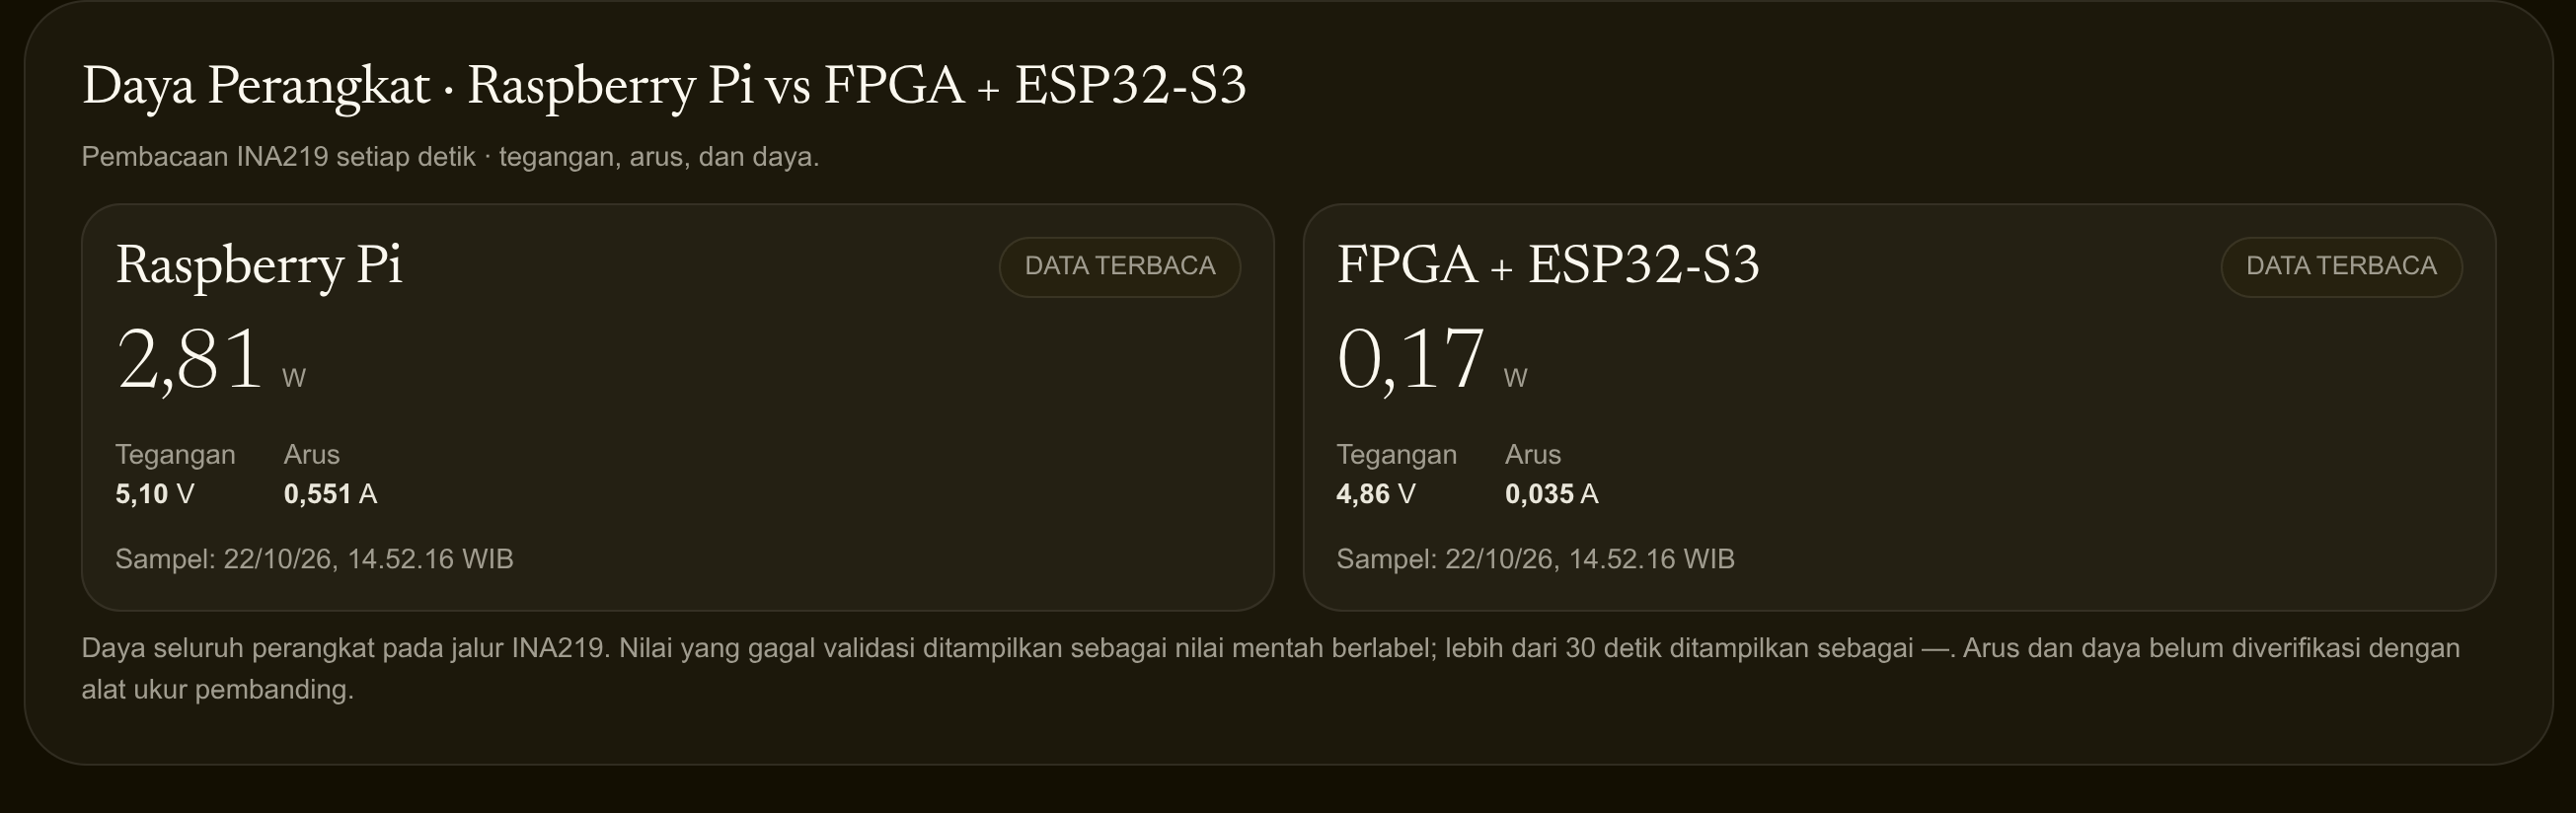
\includegraphics[height=2.15cm]{dash-daya.png}
\end{frame}

\begin{frame}{Status purwarupa: terbukti vs siap diperluas}{LAMPIRAN H}
\fontsize{7.5}{9.5}\selectfont
\renewcommand{\arraystretch}{1.3}
\begin{tabularx}{\linewidth}{@{}p{4.3cm} p{2.1cm} X@{}}
\toprule
Bagian & Status & Bukti / rencana \\
\midrule
Sensor atap $\to$ MQTT $\to$ dashboard + database & \ding{51}\ live & Google Sheets (database dashboard), InfluxDB (analisis) \\
Mesin ML (prediksi, status, baterai) & \ding{51}\ live & tiap menit; tahan sensor diam dan data berlubang \\
Chip MAC4 di Tang Nano 4K & \ding{51}\ live & ESP32-S3 $\leftrightarrow$ FPGA tiap menit; HIL 5.373/5.373 \\
Ukur daya Raspi vs chip & \ding{51}\ live & INA219 + pencatat energi per prediksi \\
Baterai 12 V 50 Ah, kontrol \& pengaman & simulasi & dump load 35 $\Omega$ terpasang; baterai + relai TKT 6 (Des 2026) \\
Multi-turbin, hybrid PLTS, iklim lain & siap diperluas & arsitektur per node; latih ulang per lokasi (pilot 2027) \\
\bottomrule
\end{tabularx}
\end{frame}

\end{document}
